\documentclass{article}
\usepackage{graphicx}
\usepackage{amsmath}
\usepackage{amsfonts}
\usepackage{bookmark}
\usepackage{booktabs}
\usepackage{exercises}
\graphicspath{ {./images/4.2} }
\usepackage{indentfirst}
\usepackage{amsthm}
\usepackage{yhmath}
\usepackage{placeins}
\newcommand*{\oldneg}{\mathord{\sim}}
\newcommand\showdiv[1]{\overline{\smash{)}#1}}
\newcommand\Mydiv[1]{%
\smash{\raise.3ex\hbox{$\big)$}}\mkern-8mu
        \overline{\enspace\strut#1}}
\setlength{\tabcolsep}{5pt}
\theoremstyle{definition}
\newtheorem{definition}{Definition}

\setlength{\parindent}{.5in}
\setlength{\parskip}{12pt}
\renewcommand{\arraystretch}{2}
\newcommand{\?}{\stackrel{?}{=}}

\title{4.2 Answers}
\begin{document}
\maketitle

\section*{1}
The initial amount is $1250$, the decay factor is $0.85$, and the percent decrease is $0.15$.

\section*{2}
A function $y=b^x$ is an exponential growth function if $b>1$, and it is an exponential decay function if $0<b<1$. Thus, to tell if a function is 
an exponential growth or decay function, we only need to check the value of $b$.

\section*{3}
Exponential decay.

\section*{4}
Exponential growth.

\section*{5}
Exponential growth.

\section*{6}
Exponential decay.

\section*{10}
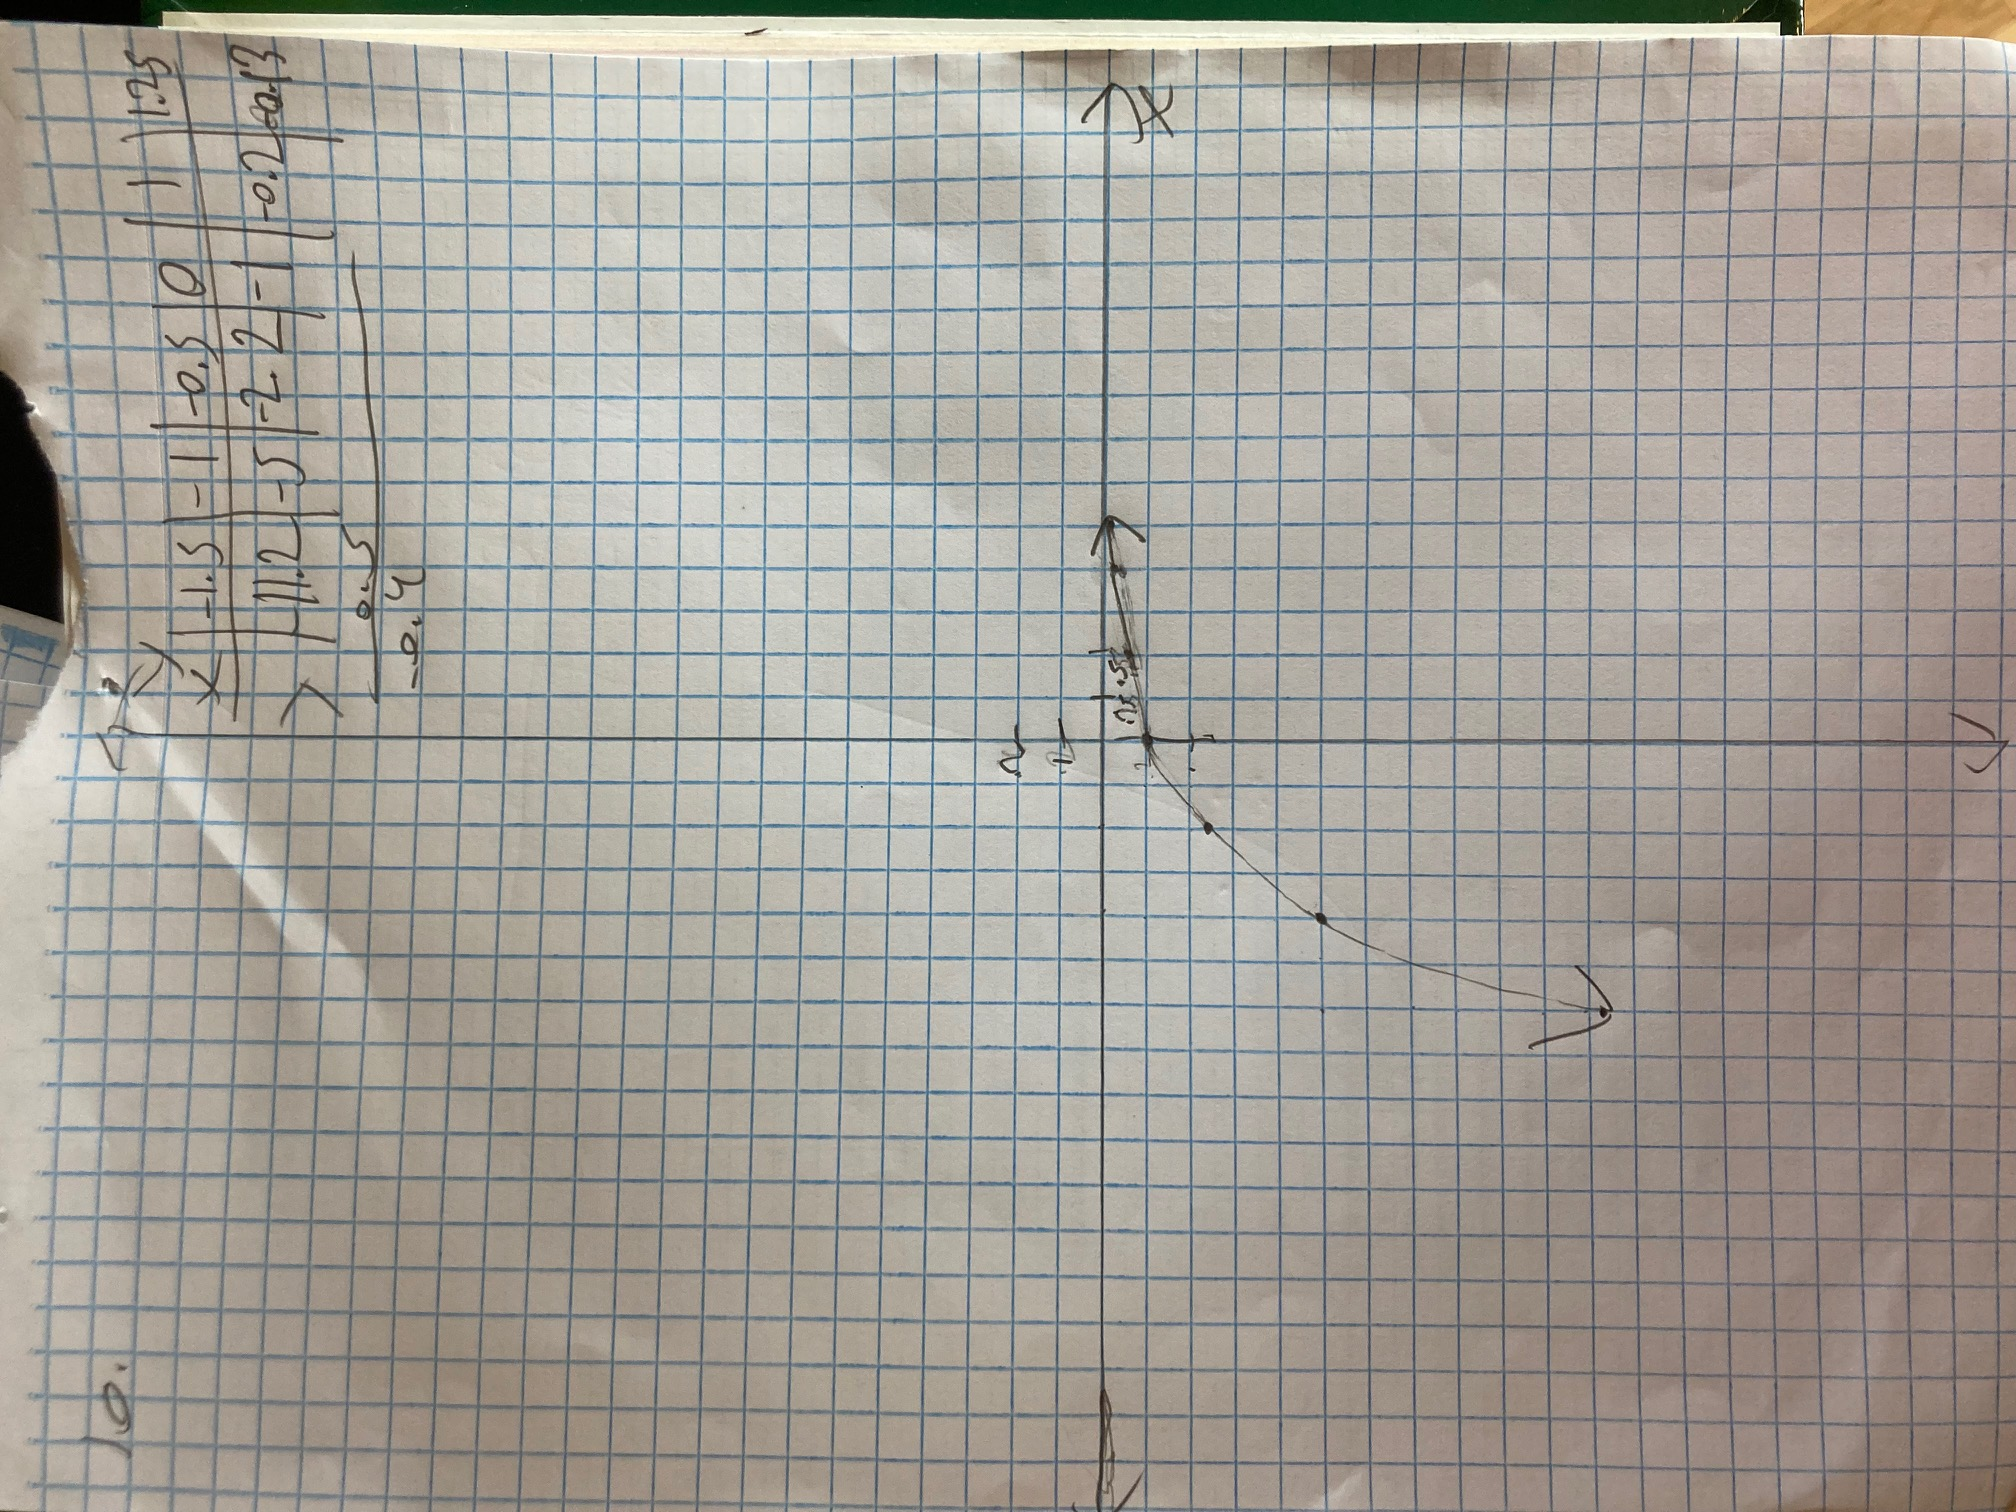
\includegraphics[width = 4in, height = 4in, angle=-90]{10}
\newline The domain of this function is all real numbers, while the range is $-\infty <x<0$, as the asymptote of this graph is $y=0$.

\section*{15}
B

\section*{23}
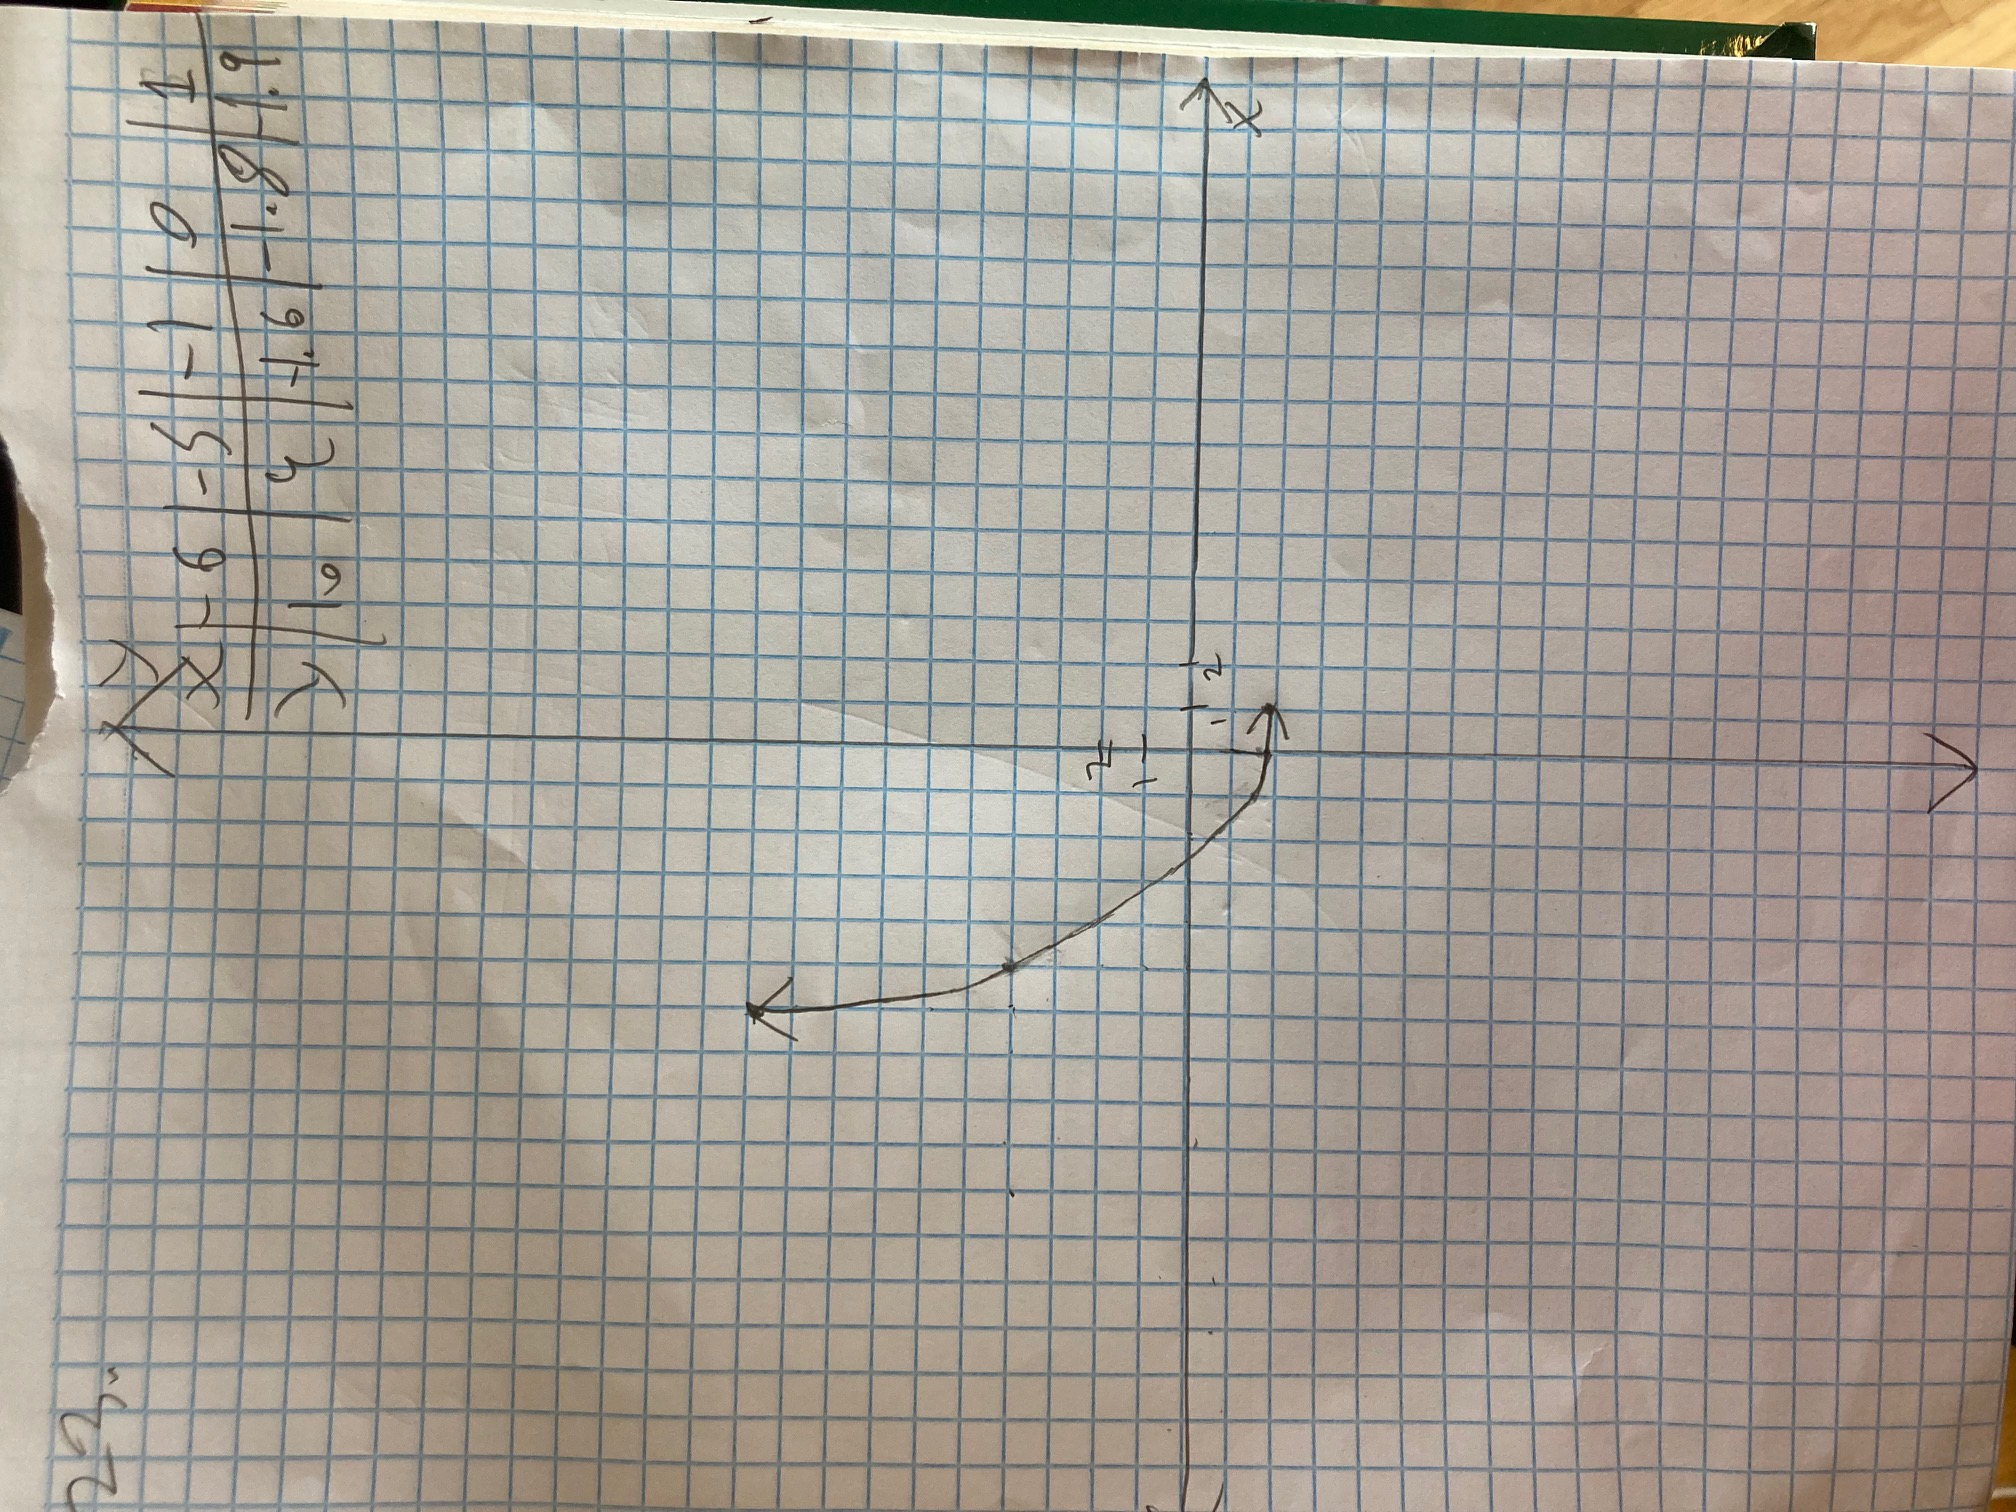
\includegraphics[width = 4in, height = 4in, angle=-90]{23}
\newline The domain of this function is all real numbers, while the range of the function is $-2<x<+\infty$, as the asymptote of this graph is 
$y=-2$.

\section*{26}
The error here is that, instead of writing $1-0.02$ as the decay factor, $0.02$ was written (the answer forgets to subtract the percent decrease 
from 1). Thus, the correct answer is that $y=500(0.98)^t$.

\section*{27}
D

\section*{28}
We need to find a function $f(x)$ such that $f(x)>(0.5)^x$, and such that $f(x)<(0.25)^x+3$. One such function is 
$y=(0.5)^x+1$.

\section*{29}
Suppose they represented the same function:
\[ 5(4)^{-x}=5(0.25)^x \] \[ 4^{-x}=0.25^x \] \[ \frac{1}{4^x}=(\frac{1}{4})^x=\frac{1}{4^x} \] thus meaning that these two graphs do represent the same 
function.

\section*{35}
(a): The decay factor is $0.89$, while the percent decrease is $0.11$.\newline
(b): \newline 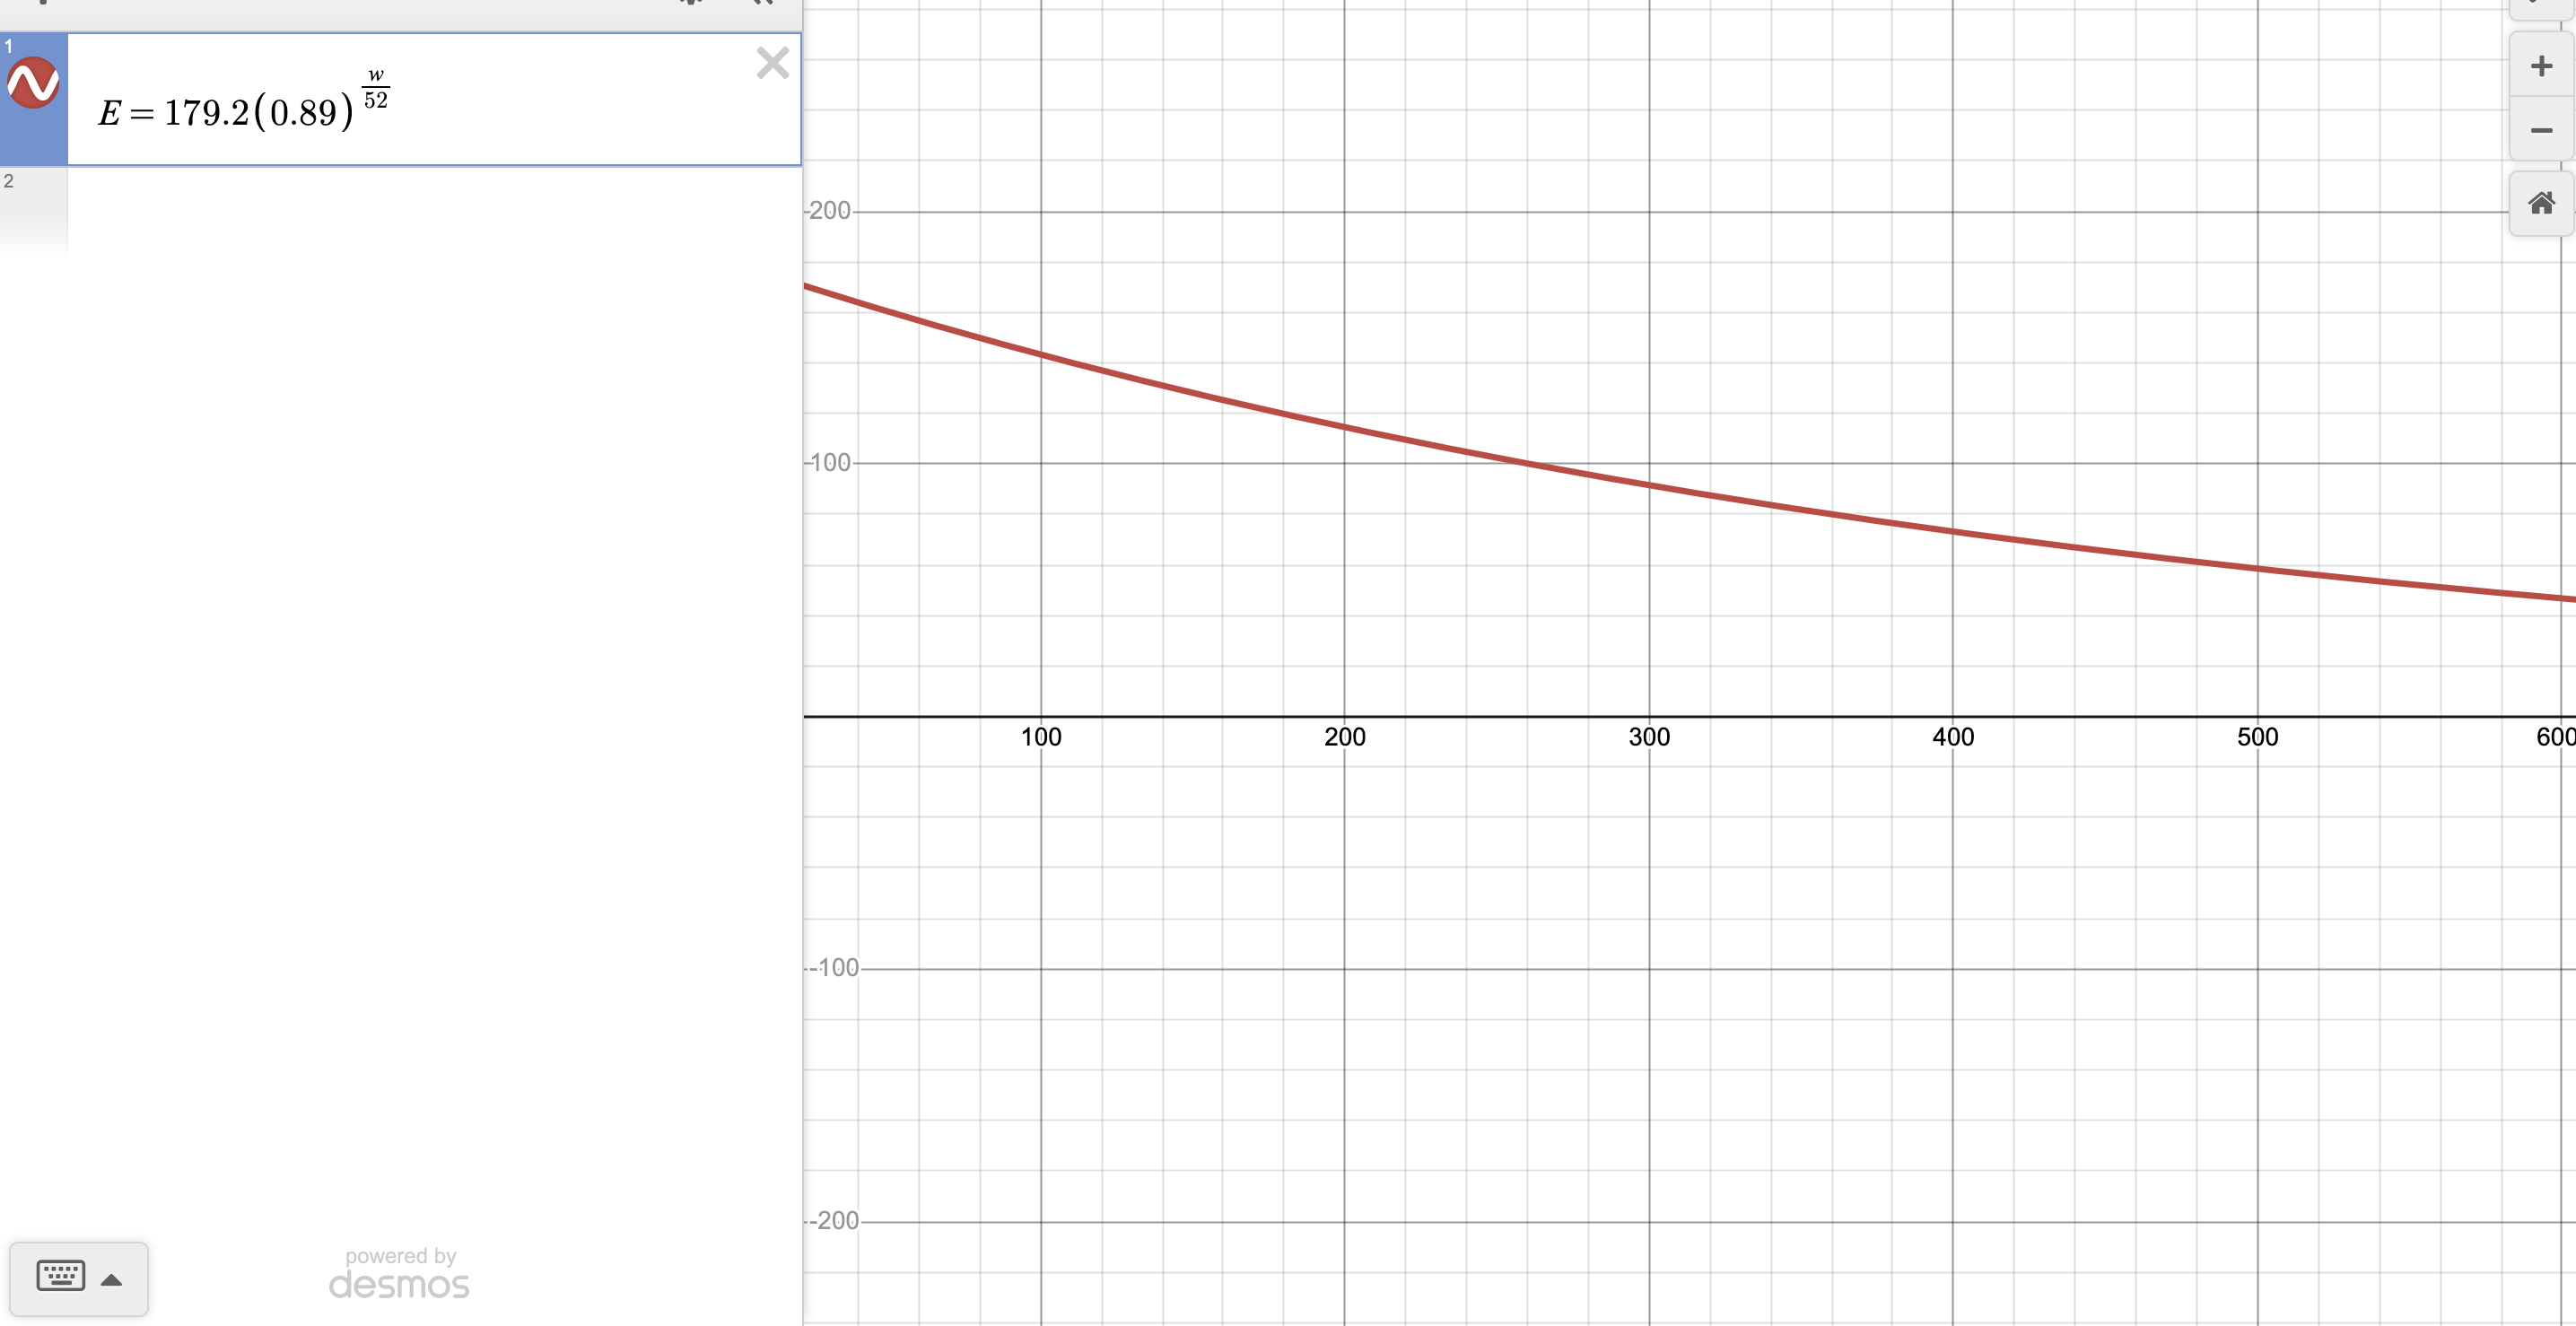
\includegraphics[width = 4in, height = 4in]{35} \newline
(c): There are about 52 weeks in a year, meaning $2.5$ years is about $52\times 2.5=130$ weeks, meaning $w=130$ in this case. Thus, the egg production 
would be about $179.2(0.89)^\frac{130}{52}\approx 134$\newline
(d): Let $g(x)=x\times 52$, which represents the number of weeks in a given number of years $x$. Thus, a function to rewrite the given equation so that time 
is measured in years would be:
\[ f(g(x))=f(52x)=179.2(0.89)^\frac{52x}{52}=179.2(0.89)^x \] 

\section*{36}
We know the initial price, as well as the price after $4$ years, meaning we can find the percent decrease:
\[ 275=1300(1-r)^4 \] \[ \sqrt[4]{\frac{11}{52}}=1-r \] \[ r=1-\sqrt[4]{\frac{11}{52}} \]
thus meaning a model for $V$ the resale value as a function of time $t$ is:
\[ V=1300(1-(1-\sqrt[4]{\frac{11}{52}}))^t=1300(\sqrt[4]{\frac{11}{52}})^t \]

\end{document}
